\section{A Framework for Scalability Testing}

The Scalability Testing Framework aims at assisting the scalability explorer, the person who tests the scalability, to verify the scalability of an application. He/She must follow some steps to verify its scalability:

\begin{enumerate}
\item Choose the variables of the problem complexity, the performance, and the architecture;
\item Define the functions of the complexity size of the problem, performance metric, and the architecture capability;
\item Choose initial values for these variables;
\item Execute the application with these initial values and obtained the initial value of the performance metric;
\item Execute multiple times with the same process and collect the performance metric for each execution;
\item Analyze the performance metric.
\end{enumerate}

To support the scalability explorer, the Scalability Testing Framework automate the steps 4 and 5, and assist the analysis of the performance metric obtained (Step 6). It has been developed in Java and it may be used with it or with languages that run on the JVM (Java Virtual Machine) and can be used with Java Annotations, such as Scala.

Since the scalability explorer needs to execute multiple times the same process by only changing the variables that define the complexity size of the problem and the architecture capability, the framework provides two Java Annotations \emph{@ScalabilityTest} and \emph{@Scale} that gives the ability to the scalability explorer to execute steps 4 and 5 by only specifying one method that describes the execution and the variables that needs to change for each execution.

\lstset{caption={Scalability test method template},label=MethodTemplate}
\begin{lstlisting}
@ScalabilityTest(scalabilityFunction=<ScalabilityFunction>, steps=<Integer>)
public List<Number> methodName(@Scale Number parameterScale, Object parameter) {
	//execution process
	return performanceMetrics;
}

\end{lstlisting}

The template of the method that is executed by the framework is shown in snippet \ref{MethodTemplate}. The annotation \emph{@ScalabilityTest} has two parameters: \emph{scalabilityFunction} and \emph{steps}. The \emph{steps} parameter defines how many times the method will be executed, we call each execution as a \emph{step}.

With the \emph{scalabilityFunction} parameter, the scalability explorer specifies how the method parameters with the annotation \emph{@Scale} will increase for each step. The parameter specified is a class that extends the ScalabilityFunction class. The classes available are \emph{LinearIncrease}, \emph{ExponentialIncrease}, and \emph{QuadraticIncrease}, which are described with more details below.

The framework collects the performance metric of each step as a list of values. After each execution, it calculates the mean and the standard deviation of these lists to plot them in a graph.

\subsection{Example}

Supposed that we developed a web service which is located in a cloud environment and we want to verify its \emph{load scalability}. Therefore, we choose the number of requests per second to be the function of the complexity size of the problem, the number of nodes which the web service is running upon, and the average response time as the performance metric. Code \ref{TestExample} shows an example of scalability test in this case.
\lstset{caption={Scalability test example},label=TestExample}
\begin{lstlisting}
@ScalabilityTest(scalabilityFunction=LinearIncrease.class, steps=5)
public List<Long> scalabilityTest(@Scale int requests, @Scale int numberNodes) {
	List<Long> resposeTimes = new List<Long>();
	instatiateNumberOfNodes(numberNodes); // Change the number of nodes
	responseTimes = makeRequestsPerSecond(requests);//Returns a list of response times
	return responseTimes;
}
\end{lstlisting}

At Line 1, we described that this method is a scalability test which must be execute 5 times  and the parameters with the \emph{@Scale} annotation should increase linearly. At Line 4, we call a method that will change the number of nodes where the web service is deployed. Then, at Line 5, we call a function that makes a number of requests per second to the web service and returns the response times of each execution.

The framework will execute the scalability test with the call presented in the Code \ref{ScalabilityTestCall}. The object \emph{wsScalabilityTest} is the one where the test is described, the string \emph{"scalabilityTest"} is the name of the scalability test, and the integers \emph{1000} and \emph{1} are the initial values of the test parameters.
\lstset{caption={Scalability test call},label=ScalabilityTestCall}
\begin{lstlisting}
ScalabilityReport report;
report = ScalabilityTesting.run(wsScalabilityTest, "scalabilityTest", 1000, 1);
\end{lstlisting}

The Sequence Diagram \ref{sequenceDiagramExample} shows the how the example above will be executed by the framework. It will execute 5 times, increasing the test parameters linearly, collecting the results, and calculating the mean and the standard deviation for each execution step. After the execution, the framework return a \emph{ScalabilityReport} object where contains the information about the execution.

\begin{figure}[hbt]
\begin{center}
	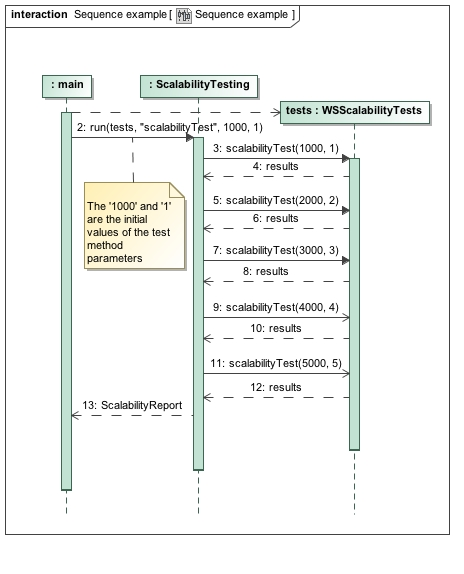
\includegraphics[scale=0.7]{images/sequenceExample.jpg}
\caption{Sequence Diagram of the Example \ref{ScalabilityTestCall}}
\label{sequenceDiagramExample}
\end{center}
\end{figure}

Code \ref{GraphPlotExample} shows how to use the report to plot a graph using the \emph{ScalabilityReportChart}. Since it can plot more than one scalability test for comparisons, it receives a list of reports. The scalability explorer can also specify the label for the performance metric axis, which is by default \emph{"Performance metric"}. Image \ref{graphIllustration} shows a graph illustration of the example above.

\lstset{caption={Graph plotting example},label=GraphPlotExample}
\begin{lstlisting}
ScalabilityReportChart chart = new ScalabilityReportChart();
List<ScalabilityReport> reports = new ArrayList<ScalabilityReport>();
reports.add(report);
chart.createChart(reports, "average response time (ms)");
\end{lstlisting}

\begin{figure}[h]
\begin{center}
	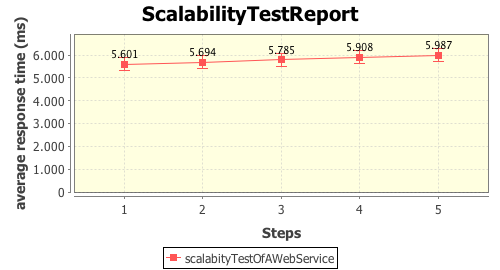
\includegraphics[scale=0.7]{images/graphExample}
\caption{Graph Illustration}
\label{graphIllustration}
\end{center}
\end{figure}

\subsection{Architecture}
The Scalability Testing Framework is composed by three main packages, one related to the annotations, one used to interpret the annotations and execute the scalability tests, and another to show the scalability testing report to the scalability explorer. The class diagram is presented in Figure \ref{classDiagram}.

\begin{figure}[htbp]
\begin{center}
	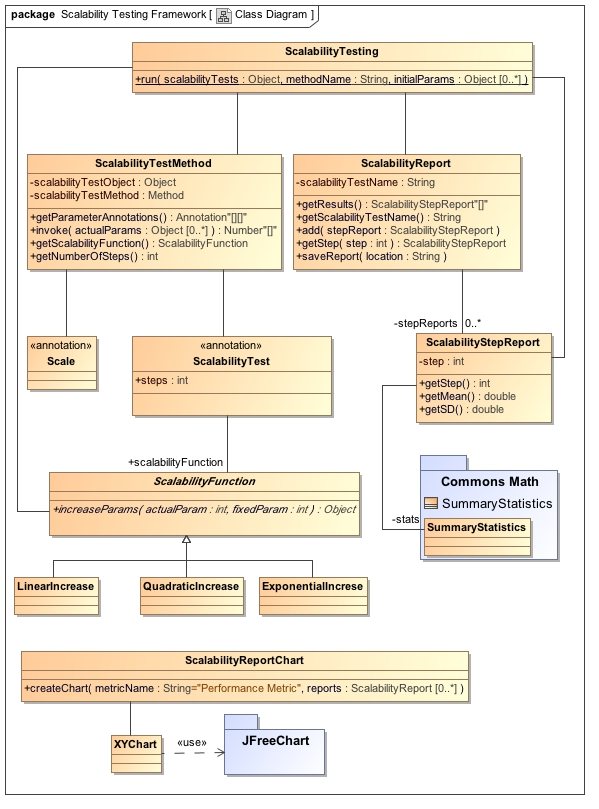
\includegraphics[scale=0.8]{images/classDiagram.jpg}
\caption{Scalability Testing Framework Class Diagram}
\label{classDiagram}
\end{center}
\end{figure}

\subsubsection{Annotations and Related Classes}
The framework provides two Java Annotations, \emph{@ScalabilityTest} and \emph{@Scale}. 

The \emph{@Scale} annotation is a parameter annotation. It must be located before the specification of the parameter and the parameter type. The parameters with this annotation will be increased by the framework in each execution step.

The \emph{@ScalabilityTest} annotation is a method annotation, which means that it must be used for methods and it is located right above the method that described a scalability test. It has two parameters. The \emph{steps} describes how many steps the framework will execute the test and must be specified. The \emph{scalabilityFunction} describes how the method parameters with the \emph{@Scale} will increase in each step. It is defined by a class that extends the \emph{ScalabilityFunction} class.

There are three ScalabilityFunction class implemented:
\begin{description}
\item[LinearIncrease] increases the parameters linearly. Thus, a parameter with initial value $x$ will be $2x$ in the second step and $nx$ in step $n$.
\item[ExponetialIncrease] increases the parameters exponentially. The parameter with initial value $x$ will be $x \times 2$ in the second step and $x \times 2^n$ in step $n$.
\item[QuadraticIncrease] increases the parameters quadratically. The parameter with initial value $x$ will be $x \times 2^2$ in the second step and $x \times n^2$ in step $n$.
\end{description}

The scalability explorer can develop another scalability function for a particular case if needed. The class must extends the \emph{ScalabilityFunction} class which has a method that receives two integers with the last value used and the initial value passed by the scalability explorer.

\subsubsection{ScalabilityTests Interpreters}
The \emph{ScalabilityTesting} class is called by the scalability explorer to execute the scalability tests. It executes them with the support of the \emph{ScalabilityTestMethod}, which interpret the annotations of the scalability tests.

For each step, a \emph{ScalabilityStepReport} is instantiated with the results. With the support of the Commons Math package, this class calculates the mean and the starndard deviation of the performance metrics.

After the execution, the \emph{ScalabilityTesting} class instantiate a \emph{ScalabilityReport} that has a list of \emph{ScalaiblityStepReport}. This class can be used by the scalability explorer to a plot a graph to analyze the results.

\subsubsection{Scalability Tests Graph}
The scalability explorer can plot the result of one or more scalability tests with their \emph{ScalabilityReport} using the \emph{ScalabilityReportChart}. This class uses the \emph{XYChart} class, that has the procedure to plot the graph with the support of the JFreeChart package.


\subsection{Implementation}